\documentclass{report}
\usepackage{graphicx}
\graphicspath{{./img/}}
\title{Week 1 - Steganography}


\author{
    Asger, Sørensen\\
    \texttt{cph-as466@cphbusiness.dk}\\
    \and
    William, Huusfeldt\\
    \texttt{cph-wh106@cphbusiness.dk}\\
   }
\date{}
\begin{document}
\maketitle

\section*{search queries}
Her er der en oversigt over alle søgninger og hjemmesider vi har været inde på for at løse opgaven. 

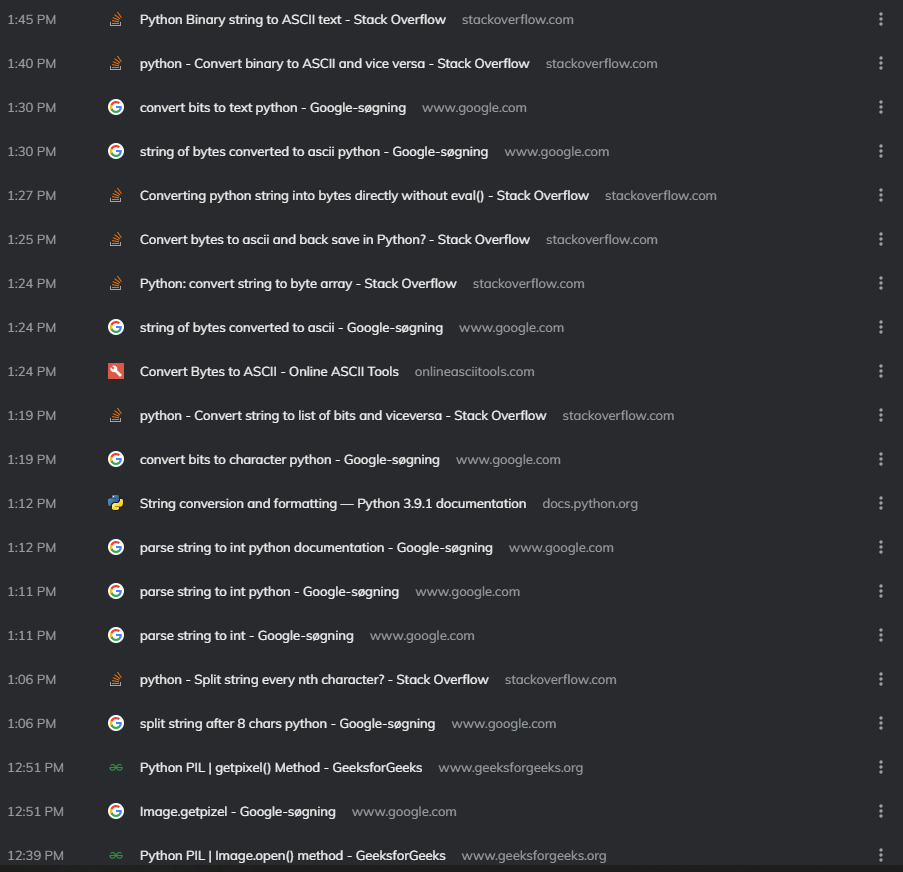
\includegraphics[height=19cm, width=15cm]{Screenshot 2021-02-10 144213.png}
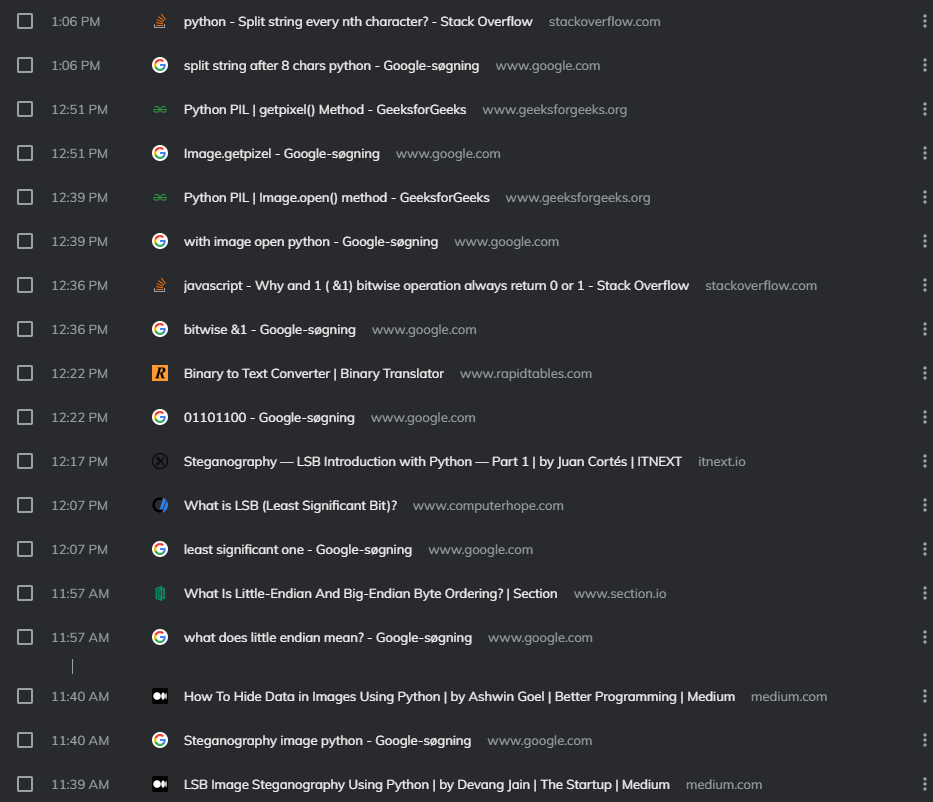
\includegraphics[height=19cm, width=15cm]{Screenshot 2021-02-10 144040.png}


\section*{Stumbling Blocks}

Vi havde meget svært ved at få forståelse for opgaven, samt hvordan det skulle løses. Det blev først meget mere forståeligt efter at vi fik undersøgt mange af de ord som vi ikke forstod, som little-endian, least significant bit, null byte samt hvordan det hang sammen med den måde som billedet er krypteret. Opgaven skulle måske have været lidt bedre formuleret, vi snakkede med en anden gruppe og de havde samme oplevelse som os.\\


Vores største udfordring var at kunne omdanne 8 bit til enkelte chars. Selv igennem en masse søgninger inde på stack overflow og google gav det virkelig mange forskellige resultater, som også skabte en masse forvirring og gjorde at vi famlede meget i tågen. Vi fandt en løsning til sidst ud fra at kombinere lidt forskelligt fra forskellige søgninger.\\

Overstående var egentlig de største udfordinger vi havde, ellers var der ikke de største udfordringer, da vi egentlig kun havde en udfordring af hvordan opgaven rent logisk skulle løses, men det fandt vi ud af mens vi var i gang med at undersøge hvad det var opgaven gik ud på. 

\section*{Diary}

12:10 - 10/02/2021
Vi er ved at undersøge hvad det er opgaven går ud på, der er stadig nogle nøgleord som vi ikke helt har forstået endnu og har svært ved at gribe hvordan det er at opgaven skal løses. \\

12:50 - 10/02/2021
Vi har fundet en start på løsningen af opgaven, og er i gang med at bruge python PIL til at få enkelte pixels og få værdierne ud af dem. \\

13:30 -10/02/2021
Vi har kunne få alle bits ud og har de værdier som vi skal bruge, men vi kan ikke få konverteret det til chars for at vi kan læse den hemmelige besked. Mange af vores google søgninger og de løsninger der er på stack overflow dækker ikke helt rigtigt over vores problematik. \\


\end{document}